\section{Results}
\label{sec:results}

\subsection{Classification Performance}
\label{subsec:classification}

Two complementary evaluation protocols are employed, consistent with the
experimental design described in Section~\ref{sec:methods}.
\emph{Cross-model statistical comparison} uses a common 503-sample
tumour-positive evaluation subset (Glioma: 162, Meningioma: 165,
Pituitary: 176) that deliberately excludes the No~Tumour class: the
3-Class CNN and 1-vs-1 Ensemble architectures are trained exclusively on
tumour subtypes and cannot predict No~Tumour, so including that class
would preclude a fair nine-model comparison~\citep{demsar2006}.
\emph{Full four-class evaluation} on the complete 703-sample test set
(additionally including 200 No~Tumour samples) is reported for the three
architectures that perform four-class prediction: the 4-Class~CNN and
both MedViT~V2 variants.

Table~\ref{tab:performance} summarises cross-model performance on the
503-sample common subset; per-class results on the full 703-sample test
set are given in Table~\ref{tab:perclass}.

\begin{table*}[ht]
\centering
\caption{Classification performance of all nine architectures on the common
  503-sample tumour-positive evaluation subset (Glioma: 162, Meningioma: 165,
  Pituitary: 176), ordered consistently with the Methods section.
  Model numbers correspond directly to those in Table~1.
  Friedman average rank (lower = better) and Bonferroni-adjusted p-values
  (§\ref{subsec:stats}) are computed on the same subset.
  Binary~CNN performs two-class (Tumour/No~Tumour) detection only.
  Accuracy is reported with 95\% Wilson score confidence intervals.}
\label{tab:performance}
\resizebox{\linewidth}{!}{%
\begin{tabular}{llcccccc}
\toprule
\# & Model & Accuracy (\%) (95\% CI) & Macro F1 (\%) & Macro AUC & Params (M) & GPU Infer.\ (ms) & Avg.\ Rank \\
\midrule
1 & Binary CNN            & 98.60 (97.2--99.3) & 98.60 & 0.999  & 1.44  & $281.6 \pm 31.3$ & 4.757 \\
2 & 4-Class CNN           & 98.01 (96.4--98.9) & 98.00 & 0.998  & 1.28  & $287.4 \pm 27.7$ & 4.945 \\
3 & 3-Class CNN           & 97.80 (96.1--98.8) & 97.80 & 0.997  & 1.28  & $270.5 \pm 27.1$ & 4.856 \\
4 & 1-vs-1 Ensemble       & 97.60 (95.9--98.6) & 97.60 & 0.997  & 3.84  & ---              & 5.053 \\
5 & ResNet-50 Dual        & 76.85 (73.0--80.3) & 76.80 & 0.952  & 26.1  & $295.2 \pm 28.6$ & 5.339 \\
6 & EfficientNet-B3 Dual  & 86.03 (82.7--88.8) & 86.00 & 0.974  & 12.8  & $294.3 \pm 30.1$ & 5.097 \\
7 & Multi-Dual System     & 93.41 (90.9--95.3) & 93.40 & 0.991  & 1.68  & $269.5 \pm 26.8$ & 4.990 \\
8 & MedViT~V2 Base        & 93.03 (90.5--95.0) & 92.80 & 0.992  & 49.31 & $289.2 \pm 26.0$ & 5.124 \\
9 & MedViT~V2 Dual        & 98.15 (96.6--99.0) & 98.13 & 0.9998 & 49.94 & $303.2 \pm 31.1$ & 4.838 \\
\bottomrule
\end{tabular}}
\end{table*}

Three performance tiers emerge. The \textbf{top tier} comprises Binary~CNN
(98.60\%), 4-Class~CNN (98.01\%), 3-Class~CNN (97.80\%), 1-vs-1~Ensemble
(97.60\%), and MedViT~V2~Dual (98.15\%). Binary~CNN achieves the highest
accuracy, but its advantage is contextual: as a two-class tumour-detector
evaluated on a 100\% tumour-positive subset, its classification task is
structurally simpler than multiclass differentiation. Among multiclass
architectures, the 4-Class~CNN and 3-Class~CNN are the most
parameter-efficient top performers (1.28~M each), while MedViT~V2~Dual
reaches comparable accuracy at roughly 39$\times$ the parameter cost
(49.94~M).

An \textbf{intermediate tier} includes the Multi-Dual~System (93.41\%) and
MedViT~V2~Base (93.03\%). Notably, the single-branch MedViT~V2 underperforms
the custom 4-Class~CNN by approximately 5 percentage points despite carrying
38$\times$ more parameters, indicating that transformer scalability does not
automatically translate to superior performance on this moderately sized MRI
dataset. The \textbf{lowest tier} is occupied by the Transfer~Learning models:
EfficientNet-B3~Dual (86.03\%) and ResNet-50~Dual (76.85\%), confirming a
persistent domain-gap between ImageNet-derived representations and brain MRI
morphology.

Per-class F1-scores from the full 703-sample test set (Table~\ref{tab:perclass})
further reveal a cross-architecture pattern in tumour-type classification
difficulty. The 4-Class~CNN achieves F1 of 98.75\% (Glioma), 97.58\%
(Meningioma), 99.26\% (No~Tumour), and 99.15\% (Pituitary).
MedViT~V2~Base scores 92.41\%, 88.02\%, 97.00\%, and 93.77\% respectively.
MedViT~V2~Dual markedly improves on the single-branch variant across all
classes: 98.76\% (Glioma), 97.21\% (Meningioma), 98.75\% (No~Tumour), and
97.78\% (Pituitary). Across all architectures, \emph{Meningioma consistently
registers the lowest per-class F1-score}, a phenomenon examined further in
Section~\ref{subsec:xai}.

\begin{table}[ht]
\centering
\caption{Per-class F1-scores (\%) evaluated on the full 703-sample test set
  (Glioma: 162, Meningioma: 165, No~Tumour: 200, Pituitary: 176) for
  four-class architectures only.}
\label{tab:perclass}
\begin{tabular}{lcccc}
\toprule
Model & Glioma & Meningioma & No~Tumour & Pituitary \\
\midrule
4-Class CNN         & 98.75 & 97.58 & 99.26 & 99.15 \\
MedViT~V2 Base      & 92.41 & 88.02 & 97.00 & 93.77 \\
MedViT~V2 Dual      & 98.76 & 97.21 & 98.75 & 97.78 \\
\bottomrule
\end{tabular}
\end{table}

\subsection{Statistical Significance Testing}
\label{subsec:stats}

The Friedman test applied to all nine models on the 503-sample common
evaluation subset yielded $\chi^2_F = 164.45$ ($p < 0.001$), decisively
rejecting the null hypothesis of equivalent performance across architectures.
The Nemenyi post-hoc test produced a Critical Difference of $CD = 0.536$ at
a family-wise significance level $\alpha = 0.05$, against which average-rank
differences are compared (Figure~\ref{fig:cd_diagram}). Only ResNet-50~Dual
(rank~5.339) lies at a distance exceeding $CD$ from the best-performing
Binary~CNN (rank~4.757), indicating that the Nemenyi test alone provides
limited discriminative resolution among the tightly clustered top models.

\begin{figure}[ht]
  \centering
  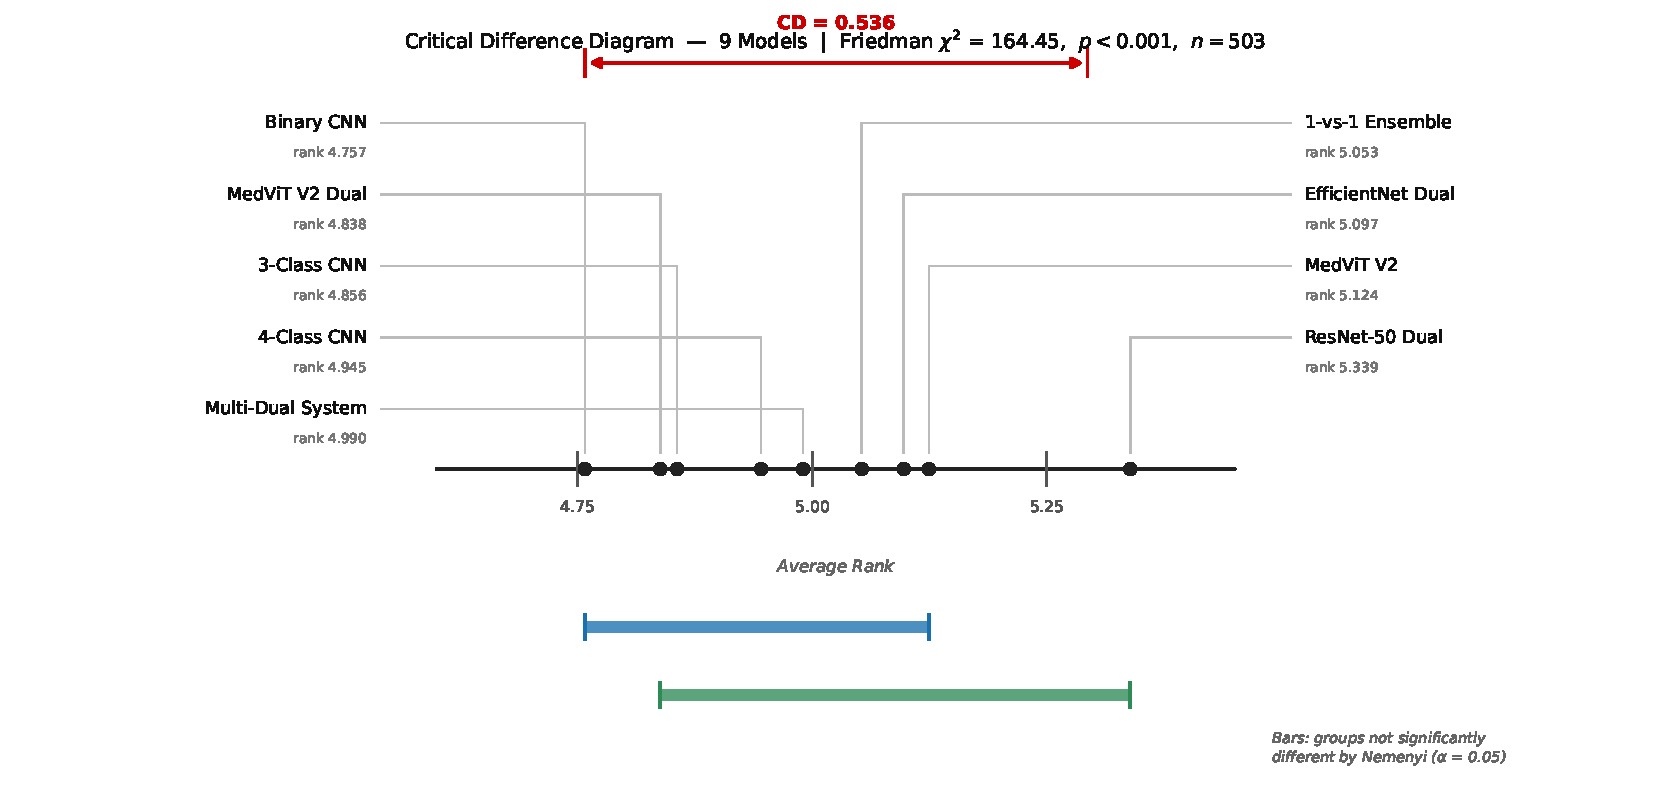
\includegraphics[width=\linewidth]{statistical_analysis_results/cd_diagram_pub.pdf}
  \caption{Critical Difference diagram for nine deep learning architectures
    evaluated on the common 503-sample tumour-positive subset (Friedman
    $\chi^2_F = 164.45$, $p < 0.001$; Nemenyi $CD = 0.536$, $\alpha = 0.05$).
    Models ranked from left (best average rank) to right (worst). Horizontal
    bars connect architectures whose average-rank difference does not exceed
    $CD$ (i.e., not significantly different by the Nemenyi criterion). Two
    overlapping groups emerge: \emph{blue} — Binary~CNN through MedViT~V2
    ($\Delta\text{rank} = 0.367$); \emph{green} — MedViT~V2~Dual through
    ResNet-50~Dual ($\Delta\text{rank} = 0.501$). Only Binary~CNN and
    ResNet-50~Dual are separated by more than $CD$.}
  \label{fig:cd_diagram}
\end{figure}

Pairwise Wilcoxon Signed-Rank tests with Bonferroni correction were applied
to all $\binom{9}{2} = 36$ model pairs. Bonferroni-adjusted p-values are
defined as $p_{\text{Bonf}} = \min(p_{\text{raw}} \times 36,\; 1)$ and
compared to the family-wise significance level $\alpha = 0.05$; the
equivalent per-comparison threshold for raw p-values is
$0.05/36 = 0.00139$. A pair is declared significantly different when
$p_{\text{Bonf}} < 0.05$ (equivalently, $p_{\text{raw}} < 0.00139$).
The top statistical group---models not significantly different from the
overall winner Binary~CNN---comprises the 3-Class~CNN
($p_{\text{Bonf}} = 0.162$) and MedViT~V2~Dual ($p_{\text{Bonf}} = 0.240$).
MedViT~V2~Dual is a noteworthy member of this group: it significantly
outperforms the 4-Class~CNN ($p_{\text{Bonf}} = 0.019$), 1-vs-1~Ensemble
($p_{\text{Bonf}} = 4.2 \times 10^{-4}$), Multi-Dual~System
($p_{\text{Bonf}} = 3.5 \times 10^{-3}$), and MedViT~V2~Base
($p_{\text{Bonf}} = 3.5 \times 10^{-6}$), confirming that the dual-branch
fusion strategy extracts statistically meaningful gains from the transformer
backbone. ResNet-50~Dual is significantly outperformed by all other models
($p_{\text{Bonf}} < 0.05$ in all eight pairwise tests).

Cohen's $d$ effect-size analysis reveals that all pairwise differences fall in
the negligible-to-small range ($d \leq 0.53$), with the sole medium effect
observed between Binary~CNN and ResNet-50~Dual ($d = 0.528$). All pairs within
the top statistical group show negligible effect sizes ($d < 0.2$), confirming
practical equivalence among the leading architectures despite their nominal
accuracy differences. The complete $9 \times 9$ matrix of Bonferroni-adjusted
p-values is provided in Supplementary Figure~S1.

%% ── Supplementary figure reference (add to appendix / supplementary material) ──
%% \begin{figure}[ht]
%%   \centering
%%   \includegraphics[width=\linewidth]{statistical_analysis_results/wilcoxon_heatmap.png}
%%   \caption{Pairwise Wilcoxon Signed-Rank test results with Bonferroni correction
%%     ($p_{\text{Bonf}} = \min(p_{\text{raw}} \times 36,\; 1)$) across all nine
%%     architectures. Red cells indicate $p_{\text{Bonf}} < 0.05$ (significant
%%     difference). Green cells indicate $p_{\text{Bonf}} \geq 0.05$ (no
%%     significant difference). Numerical values shown are $p_{\text{Bonf}}$.}
%%   \label{fig:wilcoxon_heatmap}
%% \end{figure}

\subsection{Explainable AI Analysis}
\label{subsec:xai}

Four complementary XAI methods---Grad-CAM, SHAP~(GradientExplainer), Integrated
Gradients, and Occlusion~Analysis---were applied to one median-confidence
correctly-classified sample per available class across all multiclass
architectures (Binary~CNN excluded from per-class comparison). Median-confidence
samples were selected to represent typical rather than optimal model behaviour.

\textbf{Grad-CAM.} Custom CNN architectures (4-Class, 3-Class, Multi-Dual,
1-vs-1~Ensemble) produce spatially concentrated activation maps aligned with
clinically plausible anatomical regions. Pituitary adenomas elicit consistent
sellar-region focus; Meningioma activations cluster in para-axial extra-dural
regions across all CNN models. For MedViT~V2, Grad-CAM heatmaps extracted from
the \texttt{s4\_l1\_gfp0} convolutional projection layer ($7{\times}7$ spatial
resolution) reveal broadly distributed activations extending beyond the immediate
tumour site, reflecting the long-range self-attention characteristic of
transformer architectures. Figure~\ref{fig:xai_comparison} contrasts
representative Grad-CAM overlays for the 4-Class~CNN and MedViT~V2 across
all four tumour classes.

\begin{figure*}[ht]
  \centering
  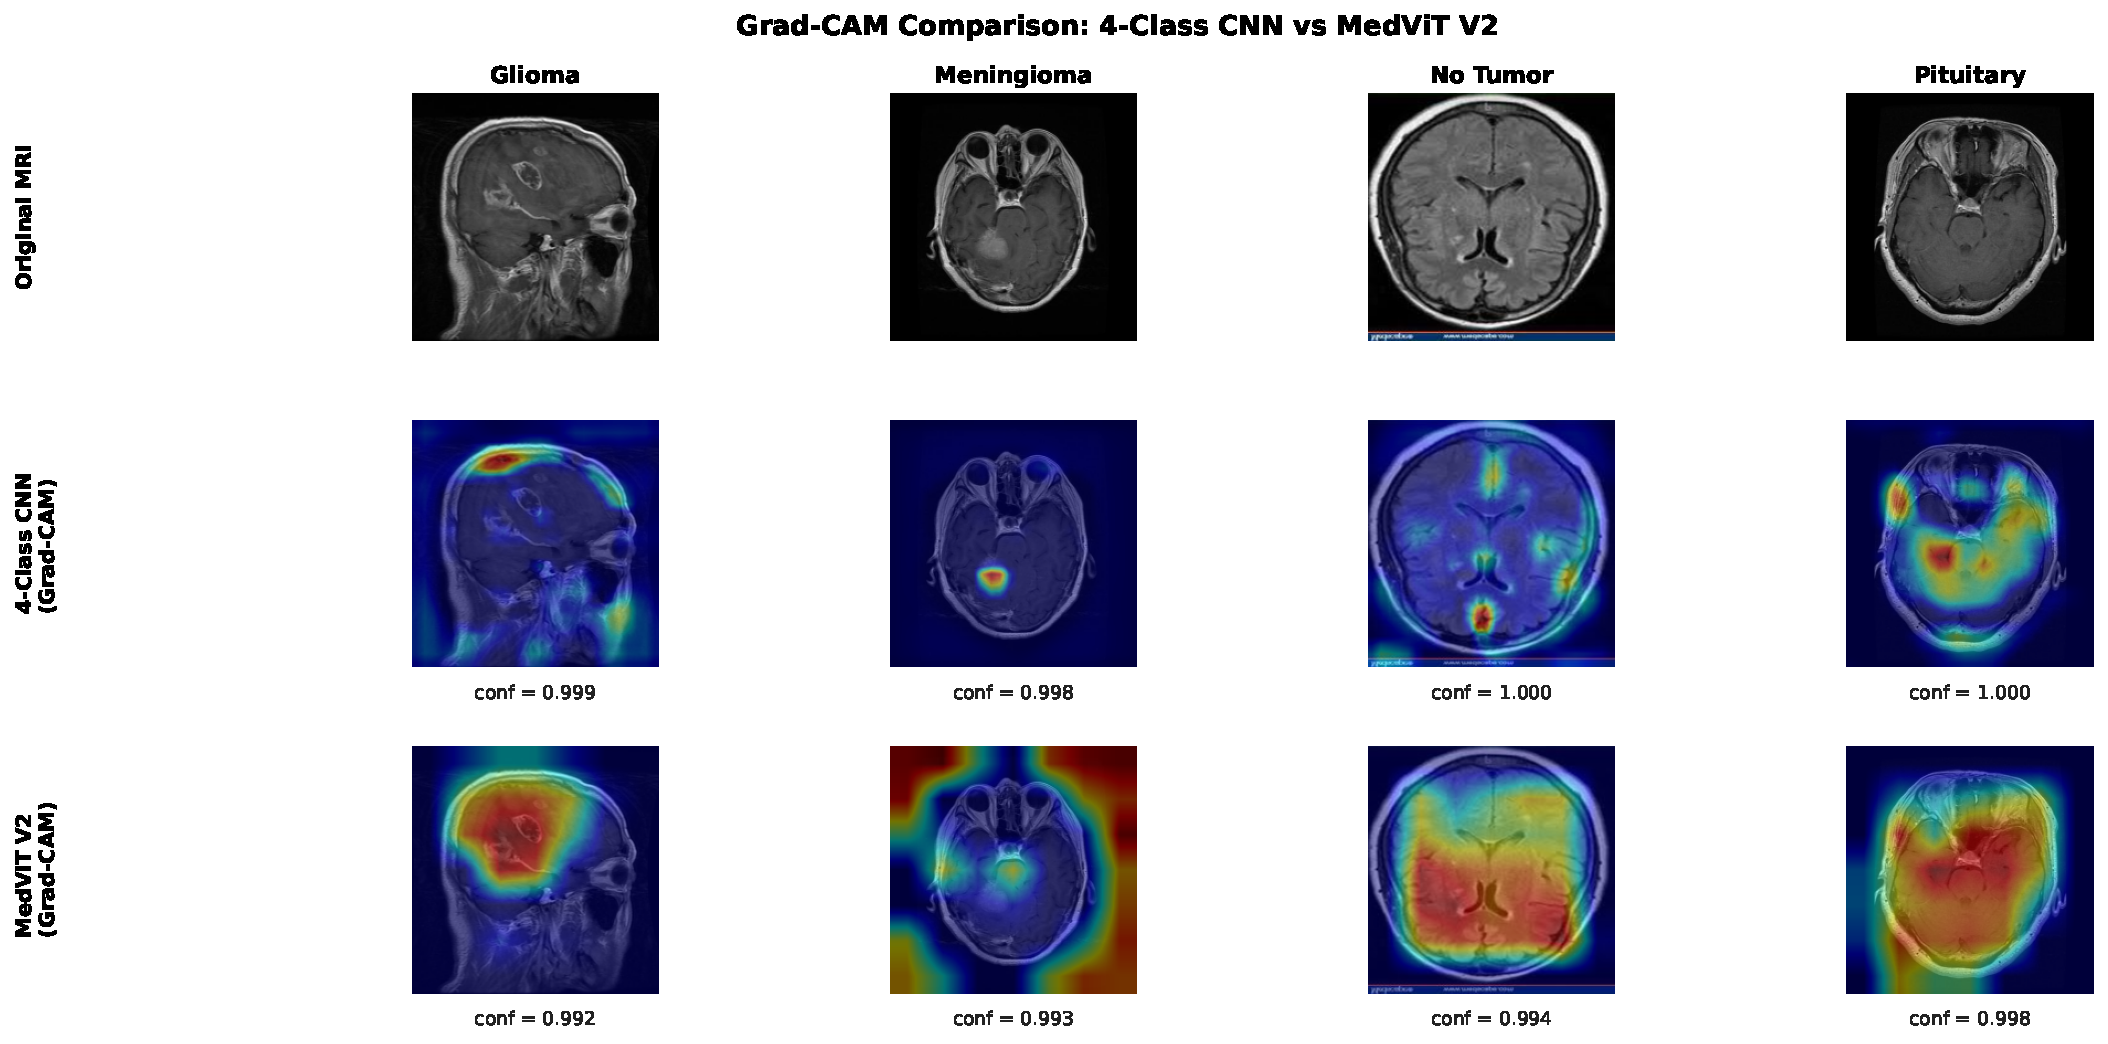
\includegraphics[width=\linewidth]{xai_comparison_cnn_vs_medvit.pdf}
  \caption{Grad-CAM activation comparison between the 4-Class~CNN
    (middle row) and MedViT~V2 (bottom row) for one median-confidence
    correctly-classified sample per class (top row: original MRI).
    CNN heatmaps exhibit spatially concentrated, lesion-focused activations
    in anatomically expected regions. MedViT~V2 heatmaps, extracted from the
    \texttt{s4\_l1\_gfp0} projection layer ($7{\times}7$ resolution), show
    globally distributed activations reflecting transformer long-range
    self-attention. Confidence values (\textit{conf}) indicate the model's
    predicted class probability for the true label.}
  \label{fig:xai_comparison}
\end{figure*}

\textbf{SHAP and Integrated Gradients.} Both gradient-based attribution methods
corroborate Grad-CAM findings for CNN architectures, delivering precise
pixel-level delineations of tumour boundaries. For MedViT~V2, both methods
produce markedly attenuated attribution magnitudes despite the model operating at
high confidence. This \emph{gradient saturation} effect---wherein transformer
networks at high-confidence operating points exhibit near-zero gradient
signals---constitutes a fundamental interpretability limitation of attention-based
architectures on this dataset and warrants consideration in clinical deployment
contexts.

\textbf{Occlusion Analysis.} Model-agnostic sliding-window occlusion
($28{\times}28$~px, stride~7) provides quantitative confidence-drop measurements
independent of internal model gradients. CNN architectures register confidence
drops exceeding 70\% when tumour-bearing regions are masked, with the Multi-Dual
System achieving a 100\% confidence drop for Pituitary tumour, reflecting the
shared backbone's specialised sellar-region representation. Occlusion
sensitivity for MedViT~V2 is distributed across a broader spatial extent,
consistent with the transformer's global context integration.

\textbf{The Meningioma Paradox.} The joint evidence from all four XAI methods
reveals a cross-architecture phenomenon: every model correctly localises the
Meningioma in its anatomically appropriate extra-axial location (convergent
evidence from Grad-CAM heatmaps, SHAP positive-contribution maps, Integrated
Gradients attributions, and occlusion confidence drops of 73--87\%), yet
Meningioma consistently records the lowest per-class F1-score across all
architectures (Figure~\ref{fig:mening_paradox}).

\begin{figure}[ht]
  \centering
  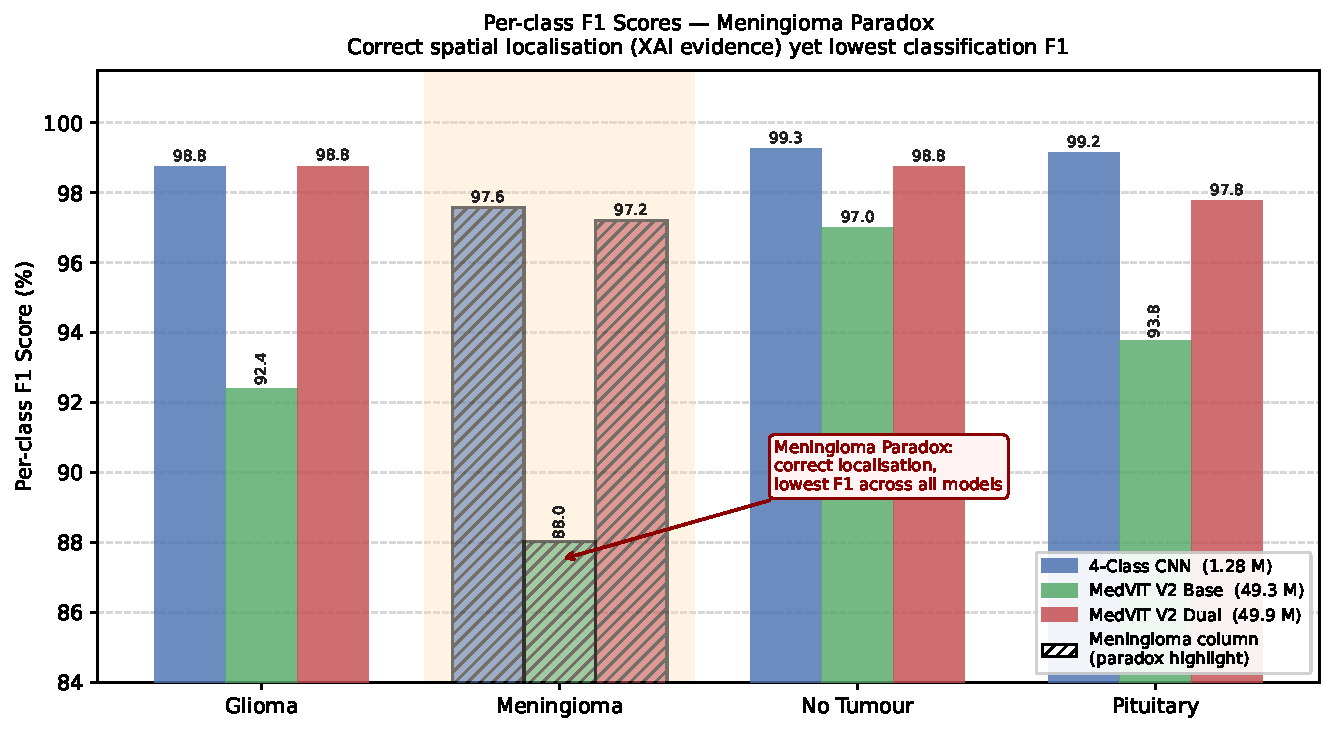
\includegraphics[width=\linewidth]{meningioma_paradox_chart.pdf}
  \caption{Per-class F1-scores for the three four-class architectures with
    detailed evaluation (full 703-sample test set). Meningioma (shaded column)
    registers the lowest F1 across all models --- 97.58\% (4-Class~CNN),
    88.02\% (MedViT~V2~Base), and 97.21\% (MedViT~V2~Dual) --- despite all
    four XAI methods confirming correct spatial localisation (Grad-CAM,
    SHAP, Integrated Gradients, and occlusion confidence drops of 73--87\%).
    This decoupling between localisation accuracy and classification F1
    constitutes the \emph{Meningioma Paradox}.}
  \label{fig:mening_paradox}
\end{figure}

This paradox---accurate spatial localisation coexisting with
relatively lower classification accuracy---is inconsistent with a detection
failure hypothesis. Rather, the XAI evidence indicates a
\emph{classification boundary problem}: Meningioma's heterogeneous morphology
and variable anatomical presentation (para-meningeal, sphenoidal) generate
feature vectors that overlap with those of other tumour classes at the final
classification layers, despite correct tumour localisation at intermediate
representations. This finding highlights the diagnostic value of XAI analysis
as a complement to accuracy metrics: a model can reliably detect where a
pathology is located while simultaneously encountering difficulty in determining
which subtype it represents.

\subsection{Ablation Study: MedViT~V2 Dual-Branch Design}
\label{subsec:ablation}

Table~\ref{tab:ablation} isolates the contribution of each architectural
component in the MedViT~V2~Dual system by comparing four configurations that
share the same evaluation protocol (503-sample common subset).

\begin{table}[ht]
\centering
\caption{Ablation of the MedViT~V2~Dual architecture. Accuracy reported on
  the 503-sample tumour-positive evaluation subset. $\Delta$ is relative to
  the 4-Class~CNN baseline.}
\label{tab:ablation}
\begin{tabular}{llcc}
\toprule
System & Branches & Accuracy (\%) & $\Delta$ \\
\midrule
4-Class CNN       & CNN only                    & 98.01 & baseline  \\
MedViT~V2 Base    & Transformer only            & 93.03 & $-$4.98pp \\
Multi-Dual System & CNN + CNN + fusion          & 93.41 & $-$4.60pp \\
MedViT~V2 Dual    & Transformer + CNN + fusion  & 98.15 & $+$0.14pp \\
\bottomrule
\end{tabular}
\end{table}

Three conclusions follow directly from Table~\ref{tab:ablation}.
First, dual-branch fusion alone does not drive performance: the Multi-Dual
System (CNN\,+\,CNN, 93.41\%) underperforms the single 4-Class~CNN (98.01\%),
attributable to the additional optimisation complexity introduced by the
masked loss function applied to the 3-class branch (which excludes
No~Tumour samples from gradient updates).
Second, transformer representations alone are insufficient: MedViT~V2~Base
achieves only 93.03\% as a single-branch model.
Third, the interaction between branches is \emph{synergistic rather than
additive}: combining the transformer and CNN branches in MedViT~V2~Dual
(98.15\%) recovers full CNN-level performance that neither branch achieves
independently, rather than averaging to the expected $\sim$95.5\%.
The decisive factor is the complementarity between transformer global
self-attention and CNN local feature extraction: each branch compensates for
the representational blind spots of the other.
